\chapter{玩家手册}
\section{运行和卸载方式}
针对我们的游戏,有两种方式可以运行:如果使用VS运行项目,则直接删除项目即可删除游戏;如果使用我们给出的安装程序运行项目,则需要使用安装程序卸载项目。
\subsection{使用VS运行项目}
在依照“第2章 开发环境”中的MSVC工具集版本、并选择好当前项目的配置环境(如masm32库的位置链接等)后,使用VS打开本实验项目,选择上方调试-开始执行(不调试)运行项目。
\subsection{使用安装程序运行项目}
我们使用VS自带的Setup扩展内容完成了整体项目的打包发布。打包后的压缩包名称为“Debug.zip”,解压该文件后,会生成以下文件:setup.exe可以完成项目软件的安装;.msi文件可以完成对软件的卸载以及修复。
\begin{figure}[htbp]
    \vspace{13pt} % 调整图片与上文的垂直距离
    \centering
    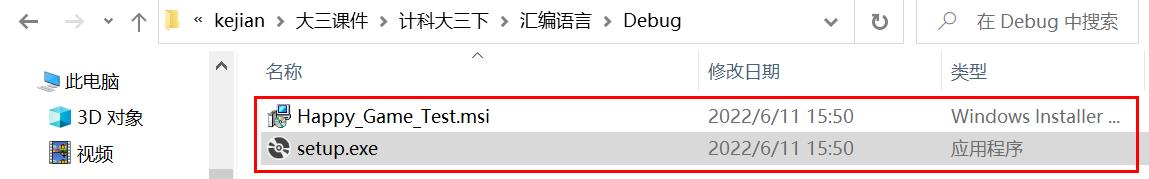
\includegraphics[width=0.8\textwidth]{images/4-1.jpg}
    \caption{解压以后的文件}% label 用来在文中索引
\end{figure}
\par
双击setup.exe,会弹出图4-2,单击“下一步”:
\par
\begin{figure}[htbp]
    \vspace{13pt} % 调整图片与上文的垂直距离
    \centering
    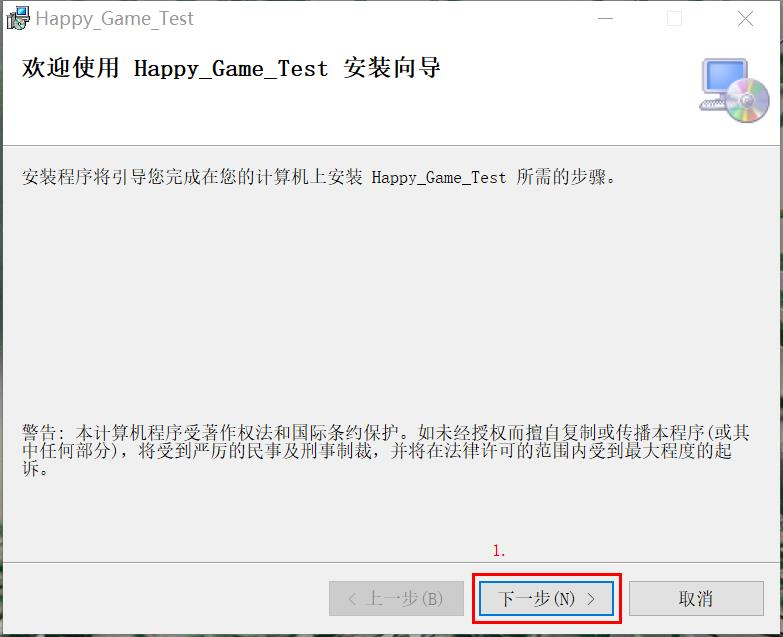
\includegraphics[width=0.5\textwidth]{images/4-2.jpg}
    \caption{安装页面}% label 用来在文中索引
\end{figure}
\par
自定义程序所在文件夹,选择“任何人”,单击“下一步”。
\par
\begin{figure}[htbp]
    \vspace{13pt} % 调整图片与上文的垂直距离
    \centering
    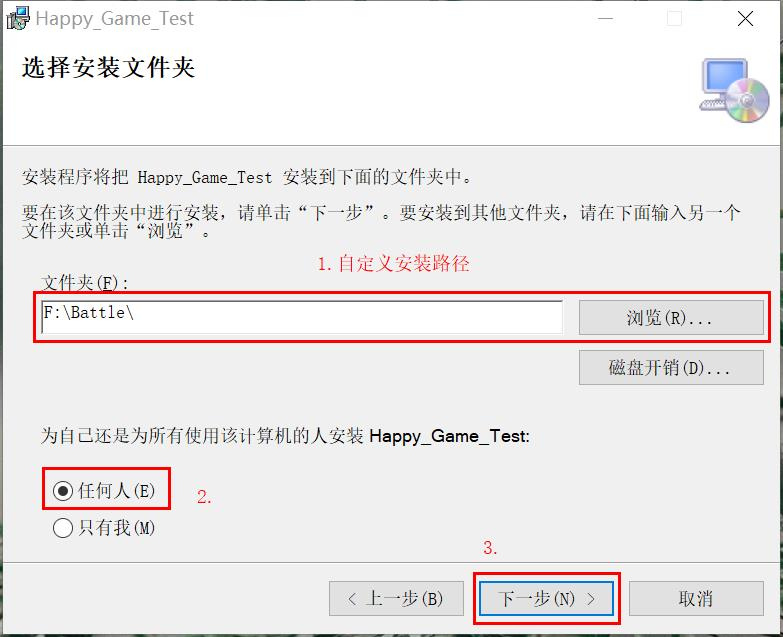
\includegraphics[width=0.5\textwidth]{images/4-3.jpg}
    \caption{选择安装路径页面}% label 用来在文中索引
\end{figure}
\par
单击“下一步”,进行安装。
\par
\begin{figure}[htbp]
    \vspace{13pt} % 调整图片与上文的垂直距离
    \centering
    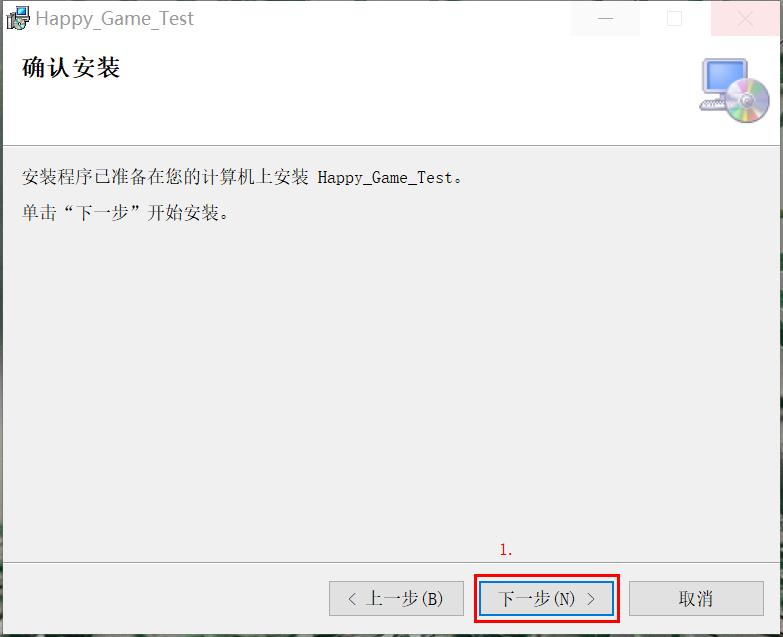
\includegraphics[width=0.5\textwidth]{images/4-4.jpg}
    \caption{确认安装}% label 用来在文中索引
\end{figure}
\par
完成安装。
\par
\begin{figure}[htbp]
    \vspace{13pt} % 调整图片与上文的垂直距离
    \centering
    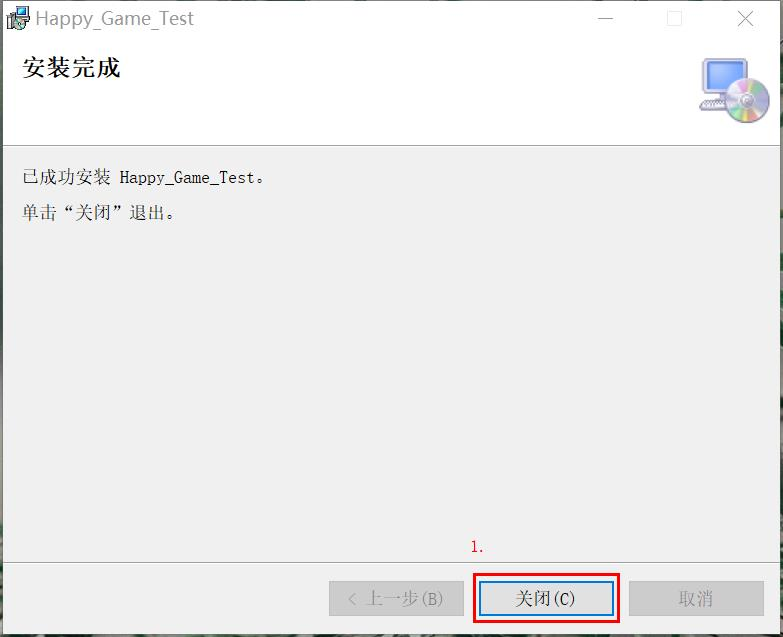
\includegraphics[width=0.5\textwidth]{images/4-5.jpg}
    \caption{安装完成}% label 用来在文中索引
\end{figure}
\par
在图4-3中自定义的文件路径里,可以找到以下文件:
\par
\begin{figure}[htbp]
    \vspace{13pt} % 调整图片与上文的垂直距离
    \centering
    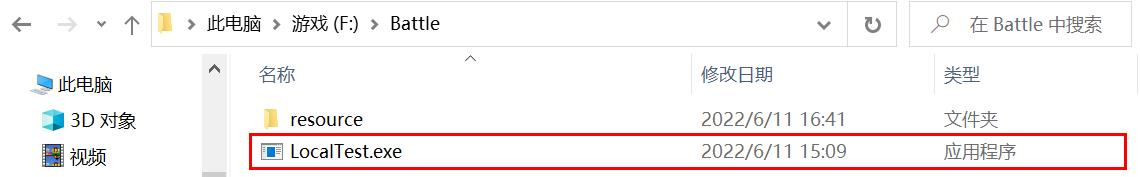
\includegraphics[width=0.8\textwidth]{images/4-6.jpg}
    \caption{生成的可执行文件}% label 用来在文中索引
\end{figure}
\par
双击“LocalTest.exe”后即可运行。
\par
在完成安装后,桌面还会生成一个快捷方式,双击快捷方式也可以直接运行游戏。
\par
\begin{figure}[htbp]
    \vspace{13pt} % 调整图片与上文的垂直距离
    \centering
    
\includegraphics[]{images/4-7.jpg}
    \caption{快捷方式}% label 用来在文中索引
\end{figure}
\subsection{使用安装程序卸载游戏}
在图4-1中,双击“.msi”格式结尾的文件,弹出图4-8。
\par
选中“删除Happy\_Game\_Test(M)”,然后单击“完成”。
\par
\begin{figure}[htbp]
    \vspace{13pt} % 调整图片与上文的垂直距离
    \centering
    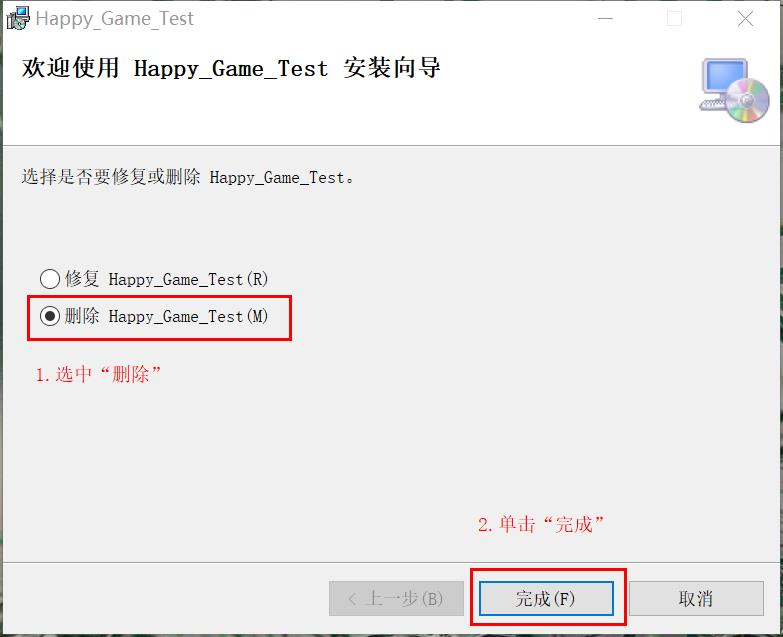
\includegraphics[]{images/4-8.jpg}
    \caption{使用安装程序删除本地已安装游戏}% label 用来在文中索引
\end{figure}
\par
在删除成功之后,单击“关闭”关闭窗口就完成了整个删除流程。
\par
\begin{figure}[htbp]
    \vspace{13pt} % 调整图片与上文的垂直距离
    \centering
    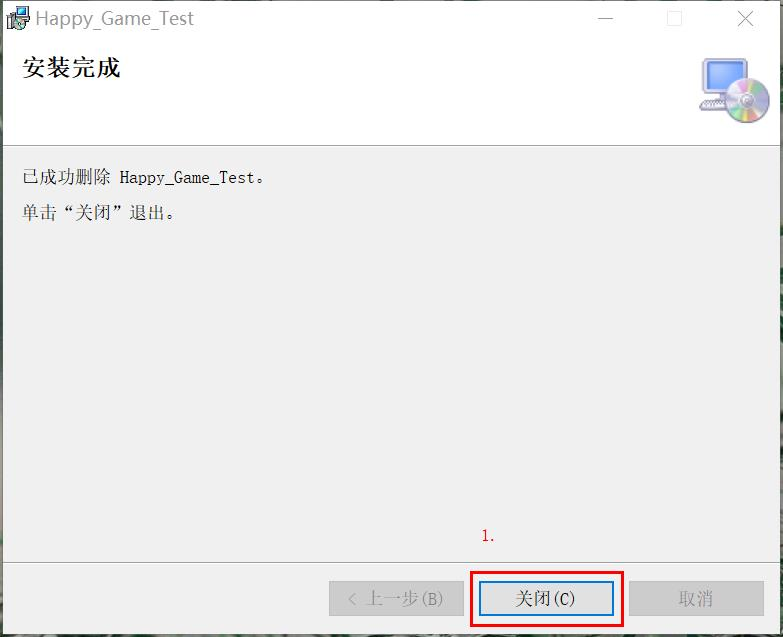
\includegraphics[]{images/4-9.jpg}
    \caption{删除成功}% label 用来在文中索引
\end{figure}
\section{运行效果与功能说明}
进入游戏后我们可以看到游戏的开始界面,其中包括Strat和Exit两个选项;点击Start我们就进入了正式游戏页面,点击Exit则会退出程序运行,关闭游戏。
\par
\begin{figure}[htbp]
    \vspace{13pt} % 调整图片与上文的垂直距离
    \centering
    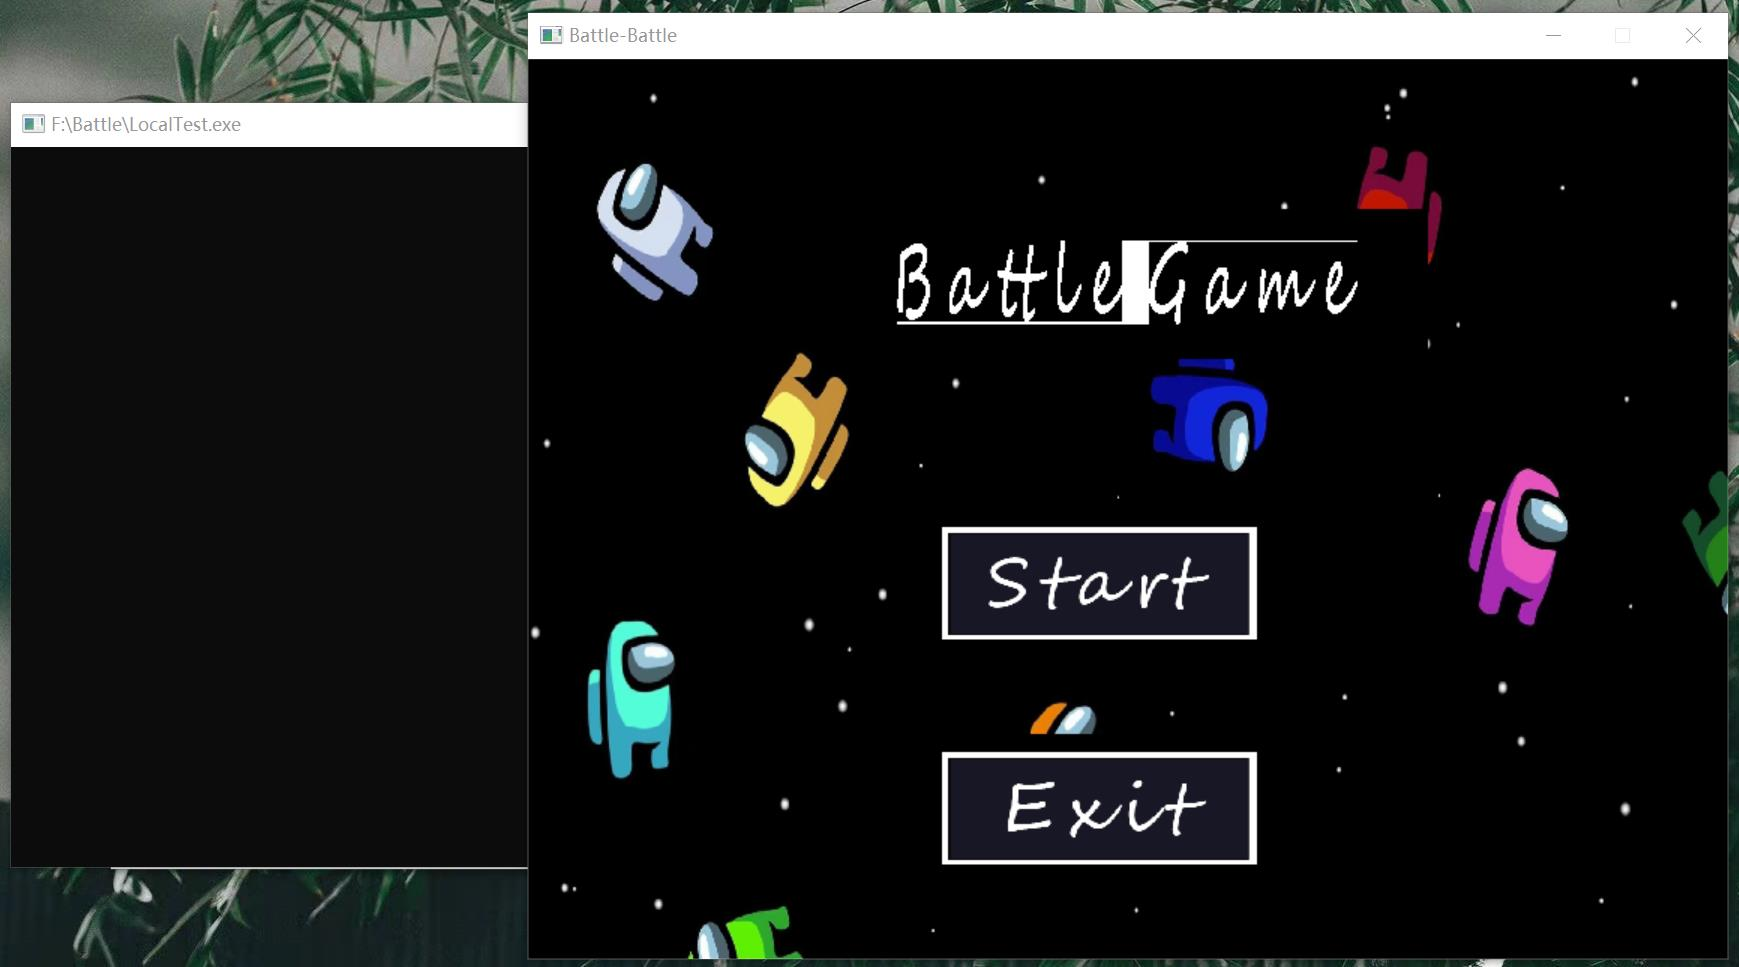
\includegraphics[width=0.8\textwidth]{images/4-10.jpg}
    \caption{游戏主菜单界面}% label 用来在文中索引
\end{figure}
\par
在游戏页面我们可以看到左右两边有两个自己移动的人物,此时游戏已经开始。游戏底部“VS”板上显示的气球代表两个玩家操作人物的生命值,在人物被击中之后生命值会依据子弹的伤害减少对应的值。
\par
\begin{figure}[htbp]
    \vspace{13pt} % 调整图片与上文的垂直距离
    \centering
    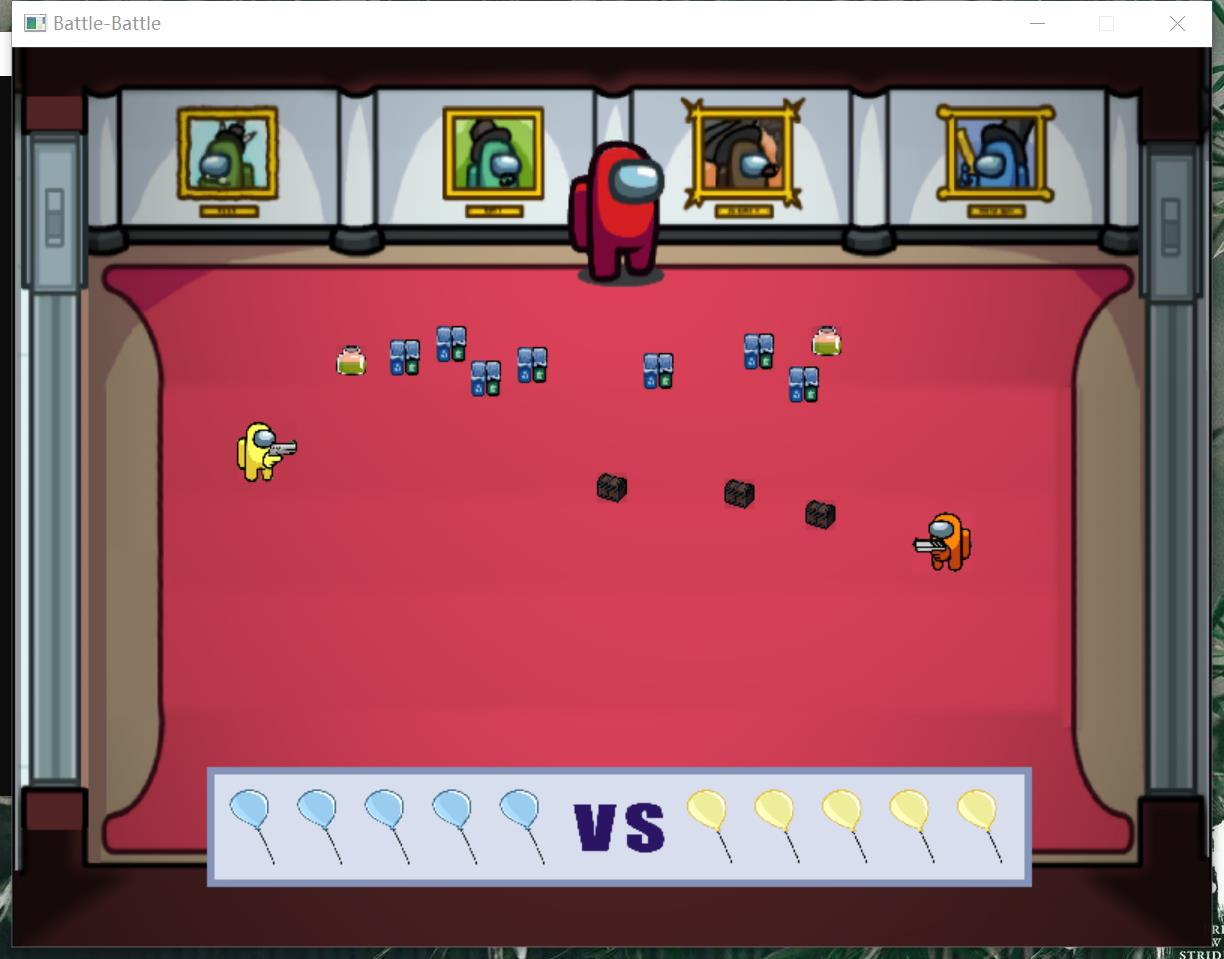
\includegraphics[width=0.8\textwidth]{images/4-11.jpg}
    \caption{正式游戏界面}% label 用来在文中索引
\end{figure}
\par
操作方式:按下键盘上的“⬅”可以让左边的人物发弹/改变移动方向;按下键盘上的“→”可以让右边的人物发弹/改变移动方向。
\par
\begin{figure}[htbp]
    \vspace{13pt} % 调整图片与上文的垂直距离
    \centering
    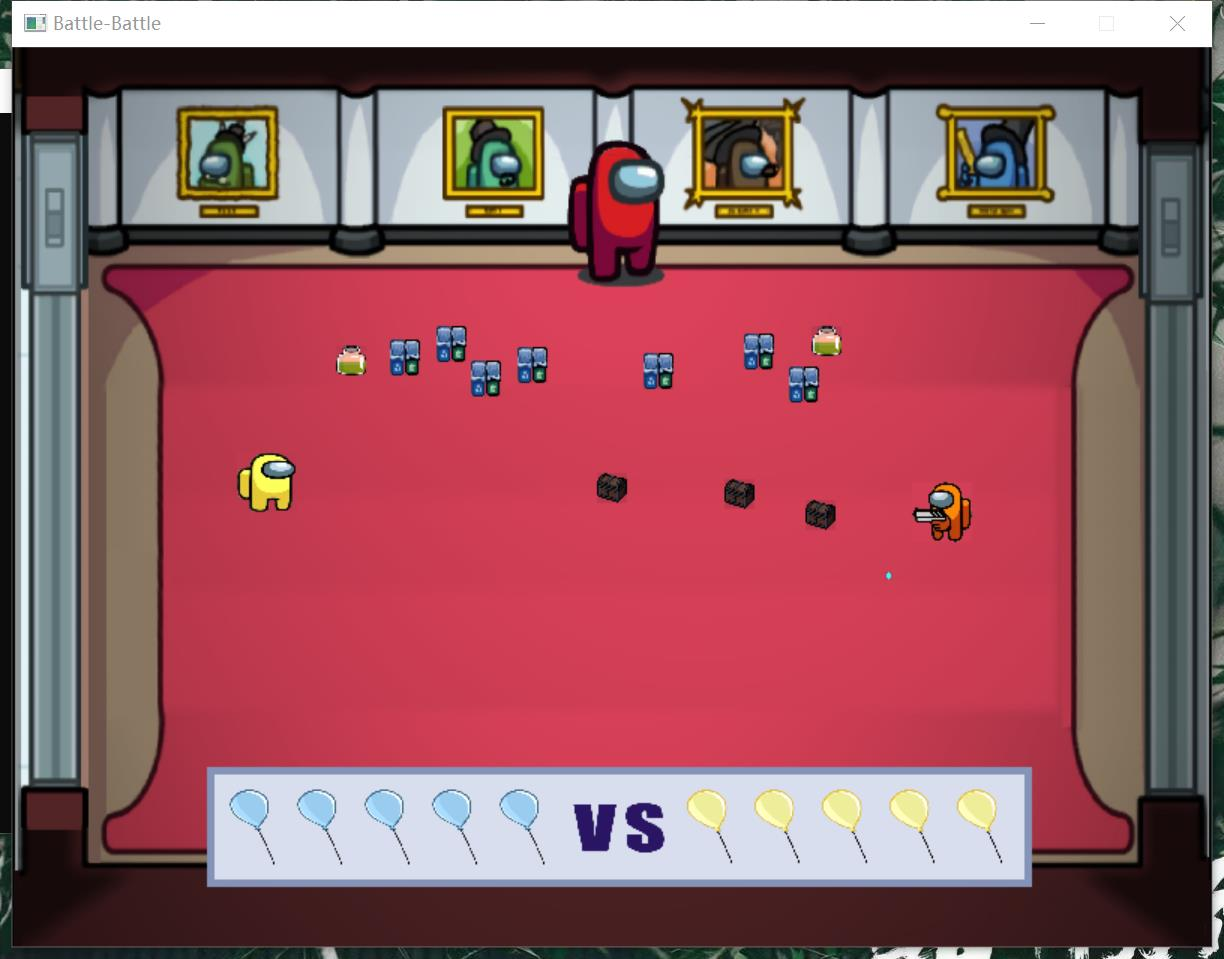
\includegraphics[width=0.8\textwidth]{images/4-12.jpg}
    \caption{Player1(黄色人物)发射子弹}% label 用来在文中索引
\end{figure}
\par
游戏规则:
\begin{itemize}
    \item 玩家每轮拥有一发子弹,在发出子弹且未装弹时,玩家只能通过“←”或“→”改变人物的移动方向;
    \item 当两名玩家均完成该轮射击后,双方同时填弹进入下一轮,填弹需要花费一定的时间。
    \item 在界面中央会随机出现若干道具,这些道具将给已发射的子弹提供属性加成,道具的功能为:\begin{itemize}
        \item 垃圾桶道具:当子弹射击到垃圾桶时,子弹会被垃圾桶弹射从而改变弹道方向;
        \item 药水道具:当子弹射击到药水道具时,子弹会得到增强,伤害提高至两点;
        \item 箱子道具:当子弹射击到箱子道具时,子弹的移动速度会降低,变化的子弹速度将影响另一位玩家的游戏节奏,从而提升对方躲避子弹的难度;
    \end{itemize}
\end{itemize}
\par
\begin{figure}[htbp]
    \vspace{13pt} % 调整图片与上文的垂直距离
    \centering
    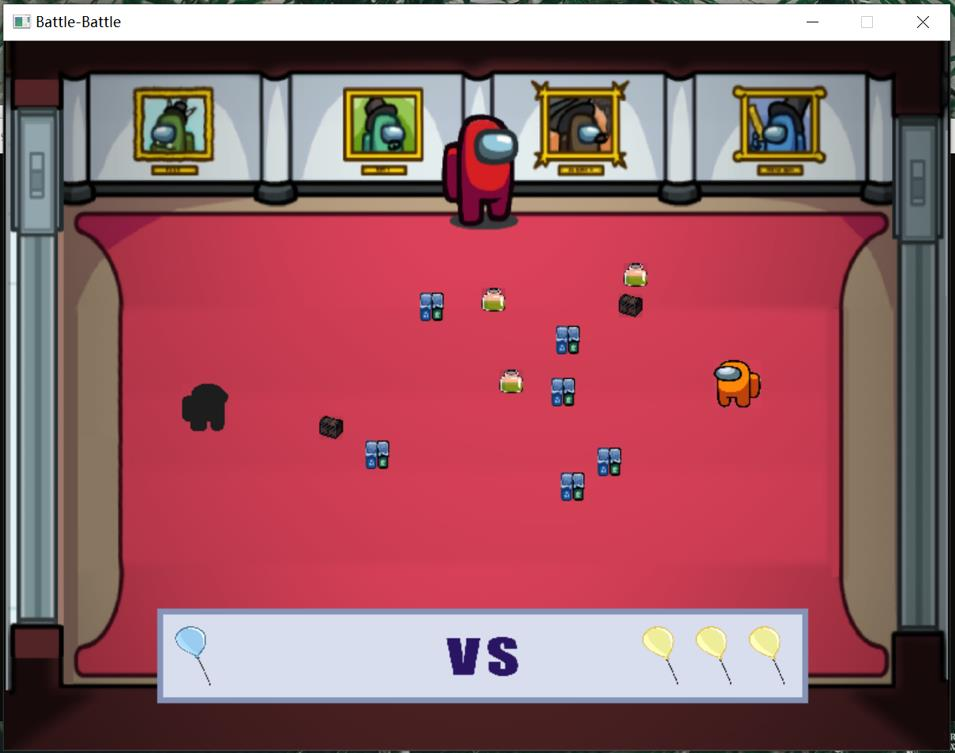
\includegraphics[width=0.8\textwidth]{images/4-13.jpg}
    \caption{Player1中弹的效果图}% label 用来在文中索引
\end{figure}
\par
当某一方的生命值小于等于0时,自动进入到游戏结算界面,游戏结束。
\par
\begin{figure}[htbp]
    \vspace{13pt} % 调整图片与上文的垂直距离
    \centering
    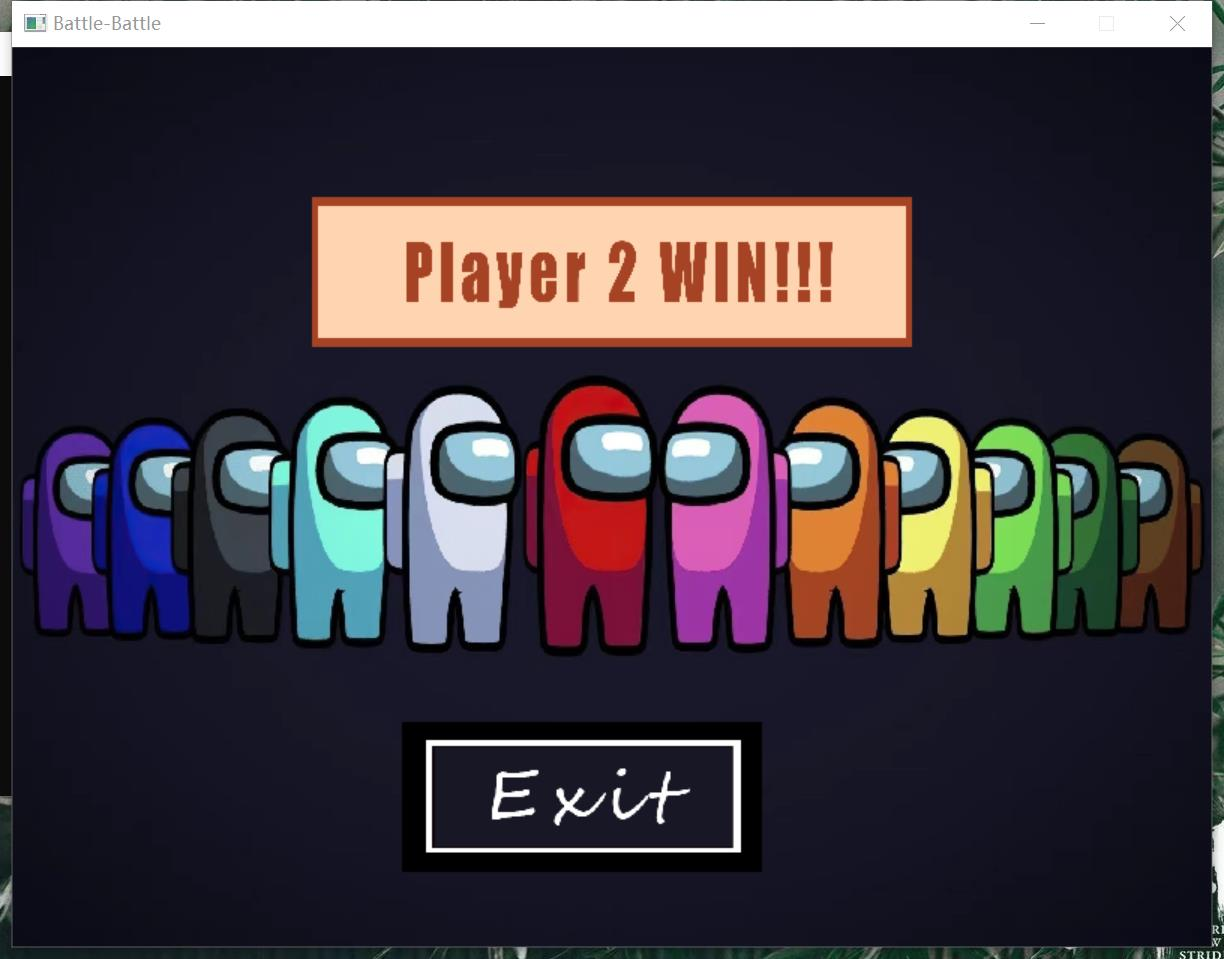
\includegraphics[width=0.8\textwidth]{images/4-14.jpg}
    \caption{Player2的获胜场景}% label 用来在文中索引
\end{figure}
\par
此时单击“Exit”即可关闭程序运行,退出游戏。

